\section{Structure of the SRG code}
Our complete SRG code is written object-oriented in C{}\verb!++! and kept as general as possible. On the one hand, this makes it easy to switch between different options of the code (e.g. use of different generators $\hat{\eta}$, harmonic oscillator or Hartree-Fock basis). On the other hand, the code is easy to extend to other systems, e.g. nuclei, and it is uncomplicated to add additional generators, potentials etc.

The specific implementations for the free-space and in-medium approach of the SRG method  are quite different. The Hamiltonian, for example, is in free space stored as complete matrix, with the matrix elements obtained by the action of creation and annihilation operators. In medium, on the other hand, it is more convenient to store the elements $f_{pq}$ and $v_{pqrs}$ separately, at the same time keeping track whether the indices correspond to hole or particle states. Since storage system, access to elements, etc. are so different for the two approaches, it makes little sense to put them into a common class. Even the implementation as subclasses of a common class \textit{Hamiltonian} seems rather artificial and forced to us. Since the same argumentation holds for other parts of the code, e.g. the classes \textit{Basis} and \textit{SRG}, we decided on two separate codes. \\
Nevertheless, we tried to find as many common data structures and methods as possible, enabling us to have 
common classes that can be used by both methods. 
To keep everything as structured and transparent as possible, we chose the same names for the classes that are specific for the two approaches. The following list summarizes the classes we designed, and gives a short explanation regarding their purpose.


\paragraph*{Classes specifying the quantum mechanical system}
\begin{itemize}
\item Class \textit{System}: A class for holding all data structures and methods of a specific system. It serves as interface for solver classes.
\item Class \textit{Hamiltonian}: A class for handling the Hamiltonian matrix in a given basis.
\item Class \textit{Basis}: A class to contain the basis which the Hamiltonian is set up in. For IM-SRG, this class is in particular responsible for creating and administering a two-particle basis.
\item Class \textit{SPstate}: A class for holding the single-particle states.
\end{itemize}
\paragraph*{Solver classes}
\begin{itemize}
\item Class \textit{SRG}: A many-body solver. It accepts an object of type \textit{System} and uses the SRG method to determine the ground state energy.
\item Class \textit{HartreeFock}: Our second many-body solver. A class for performing a Hartree-Fock calculation and transforming a given basis to  Hartree-Fock basis. The class can be used separately for solely determining the Hartree-Fock energy or combined with other solvers, if a Hartree-Fock basis is desired.
\end{itemize}

\paragraph*{Organization of code}
Our complete code lies in a folder called \textit{SRG}. This folder has the following items:
\begin{itemize}
\item Folder \textit{src}: This folder contains one subfolder for each of the above mentioned classes. Each subfolder has the name of the class and contains one header (\textit{*.h}) and one (or several) source (\textit{*.cpp}) files. 
\item Folder \textit{lib}: This folder contains header files with our specifications for use of libraries and parallelization.
\item Folder \textit{output}: This folder receives all output files that are created during a run.
\item File \textit{main.cpp}: The main file. It runs our code for one specific choice of input parameters.
\item File \textit{makeElements.py}: Python script for creating the input files with  two-particle elements from the OpenFCI \cite{Kvaalcode} library. The folder \textit{OpenFCI} should be placed next to the \textit{SRG} folder.
\item File \textit{Makefile}: Compiles our code by simply calling \textit{make}. 
\item File \textit{runSerial.py}: Python script for running the code with one specific choice for the input parameters at a time, usually several different runs after each other. The script calls the code in the OpenFCI library, creates the input files and places them in an appropriate folder, compiles the SRG code by calling the \textit{Makefile} and runs the code with correct input parameters for the main file. That way, the user does not have to deal explicitly with the previous files.
\item File \textit{runParallel.py}: Python script with the same functionality as \textit{runSerial.py}. It opens up the possibility to run simulations with different input parameters (e.g. different oscillator frequencies $\omega$) in parallel. 
\item File \textit{mainParallel.cpp}:  Wrapper that runs the main program in parallel, with the parameters specified by \textit{runParallel.py}. Parallelized with MPI (Message Passing Interface).
\end{itemize}


\section{Implementation of SRG - general aspects}
In the following, we will present the common parts of our program, before we move on and look at those parts that are specific for the free-space and in-medium implementation, respectively.
\subsection{Class \textit{System}}
The first common class is the class \textit{System}, whose task it is to hold all the data structures and methods that characterize a specific system, i.e. Hamiltonian, single-particle basis etc. That way, it shall serve as communication point for the solver, in our case the SRG method, and make the program clearly structured and organized. It contains several other classes like \textit{Hamiltonian} and \textit{Basis}, and is responsible for appropriate communication between those classes. \\
An important point is that the class \textit{System} is supposed to embed those aspects that are specific for a system, whereas \textit{Hamiltonian}, \textit{Basis}, etc., are general classes that can be used for all kinds of systems, e.g. quantum dots and nuclear systems, and in arbitrary many Euclidean dimensions. In order to have a general program that can easily be adopted to different kinds of physical problems, we have therefore constructed \textit{System} as a virtual base class, giving the possibility to implement system-specific routines in derived subclasses. \\
One example is the labelling of single-particle states: For two-dimensional quantum dots with a harmonic oscillator basis, this looks as in figure \ref{fig:shellstructure}, but already for a three-dimensional quantum dot, we would need a different mapping scheme. Therefore, the function \textit{mapping} is virtual in the class \textit{System}, and we implemented the concrete mapping of figure \ref{fig:shellstructure} in the derived subclass  \textit{System\_2DQdot}.

\begin{figure}
\begin{center}
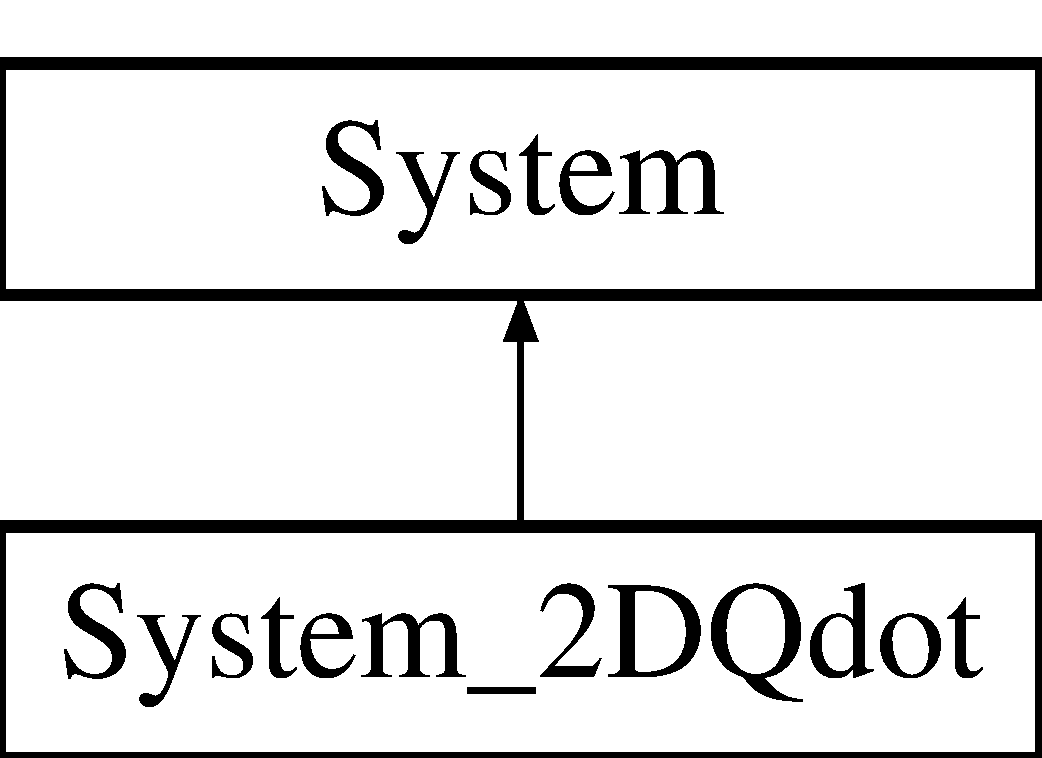
\includegraphics[scale=0.15]{../Plots/classSystem.pdf}
\end{center}
\caption{The class \textit{System} is a virtual base class, and needs to be extended by subclasses containing system-specific methods and data structures.}
\label{fig:classSystem}
\end{figure}


\subsection{Class \textit{SPstate}}
Another general class that can be used for arbitrary systems and bases is the class \textit{SPstate}. One instance of this class represents one specific single-particle state, characterized by specific quantum numbers and a single-particle energy. The basis of the Hamiltonian, e.g. a harmonic oscillator basis, which is a separate class in our program, can then contain an array of those single-particle states, with its size depending on the size of the basis.\\
Since the algorithm specifying the quantum numbers is system-dependent, we have chosen to put the mapping function, which maps between a particular single-particle state and the associated quantum numbers, into the  subclasses of \textit{System}, rather than putting it into \textit{SPstate} which should be as general as possible.\\
In the following, we demonstrate how the mapping is performed in the case of two-dimensional quantum dots, implemented in the subclass \textit{System\_2DQdot}.

\paragraph{Mapping the single-particle states for two-dimensional quantum dots}
 
Considering the shell structure of quantum dots presented in chapter \ref{chap:qdots}, a shell number $R$ corresponds to $R(R+1)$ possible single-particle states, where at least one of the quantum numbers $n,m,m_s$ is different. 
Beginning form the lowest shell, each single particle state is assigned an index $\alpha$, as illustrated in figure \ref{fig:shellstructure}. \\
We now perform a mapping
\[
\left| \alpha \right\rangle \rightarrow \left| n,m,m_s \right\rangle,
\]
such that each index $\alpha$ corresponds to a specific set of quantum numbers $n(\alpha),m(\alpha), m_s(\alpha)$. The quantum number $n$  is the nodal quantum number as given in Eq. (\ref{eq:Laguerre}), $m$ denotes the angular momentum quantum number and $m_s$ the spin projection. 
An example for a two-dimensional quantum dot and the first four shells is given in table \ref{tab:mapping3shells}. In order to make our code compatible with the OpenFCI [ref] library generating the interaction elements later on, we have slightly changed the indexing within a shell $R$.

\begin{table}
\begin{center}
\begin{tabular}{c c c c c | c c c c c }
\hline\hline
$\alpha$ & $n$ &  $m$ & $m_s$ & $R$ & $\alpha$ & $n$ &  $m$ & $m_s$ & $R$ \\
\hline
0 & 0 & 0 & 1 & 1 & 10 & 0 & 0 & 1  &\\
1 & 0 & 0 & -1 & & 11 & 0 & 0 & -1  &\\
\hline
2 & 0 & -1 & 1  & 2& 12& 0 & -3 & 1  &4\\
3 & 0 & -1 & -1 &  &13& 0 & -3 & -1  &\\
4 & 0 & 1 & 1  &  &14& 1 & 3 & 1  &\\
5 & 0 & 1 & -1 &  & 15& 1 & 3 & -1 &\\
\cline{1-5}
6 & 0 & -2 & 1  &  3& 16& 1 & -1 & 1  &\\
7 & 0 & -2 & -1 &  &17& 1 & -1 & -1  &\\
8 & 1 & 2 & 1  &  &18& 0 & 1 & 1  &\\
9 & 1 & 2 & -1 &  &19& 0 & 1 & -1  &\\
\hline\hline
\end{tabular}
\end{center}
\caption{ Overview of the mapping between single-particle states $\alpha$ and corresponding quantum numbers $n,m,m_s$ in a harmonic oscillator basis, here for the first four shells. Each state $\alpha$ has been assigned a specific set of quantum numbers with allowed values given by $n = 0,1,...$, $m = 0,\pm 1, \pm 2,\dots$ and $m_s = \pm \frac{1}{2}$, where the latter has been simplified to $m_s \pm 1$ such that only integers have to be stored.}
\label{tab:mapping3shells}
\end{table}

Studying this table and the shell structure in figure \ref{fig:shellstructure}, we observe a pattern which makes it possible to automize the assignment of quantum numbers through a mapping algorithm.\\
The first observation is that all states appear in pairs with positive and negative $m_s$, such that $m_s$ can simply be modelled by an alternating sequence. The second, more interesting point is that for each shell $R$, there exist exactly $R$ states with the same single-particle energy $\epsilon$. Looping over those $R$ states, $m$ starts with $m = 1-R$ and increasing in steps of $2$, always first with negative, then with positive sign.
That way, one ends up with the algorithm demonstrated in listing \ref{lst:mapping}, which performs the mapping for two-dimensional quantum dots and additionally computes the single-particle energies $\epsilon_i$.

\begin{lstlisting}[float,caption= {Algorithm performing the mapping $\left| \alpha \right\rangle \rightarrow \left| n,m,m_s \right\rangle$. The array \textit{qnumbers} contains the quantum numbers in the order $n,m,m_s$. Line 12, for example, then means that we access $m_s$ of the single particle state $\alpha$, contained in the Basis \textbf{Bas}.}, label=lst:mapping]
// Mapping between |alpha> and |n,m,m_s>

// Loop over all shells
for(int shell = 1; shell <=R; shell ++){
        
        m_count = 1-shell;
        
        for( int i = 0; i< shell; i++){
            
            Bas->singPart[alpha].qnumbers[1] =  Bas->singPart[alpha+1].qnumbers[1] = m_count; // m
            Bas->singPart[alpha].qnumbers[0]  = Bas->singPart[alpha+1].qnumbers[0] = i/2; // n
            Bas->singPart[alpha].qnumbers[2] = -1; // m_s
            Bas->singPart[alpha].eps = Bas->singPart[alpha+1].eps = shell*omega; //sp_energy
            alpha++;
            Bas->singPart[alpha].qnumbers[2] = +1; // m_s
            alpha++;
            if(i%2 == 0){
                 m_count *= -1; 
            }   
            else{
                m_count = -m_count +2; 
            }
        }       
    }
\end{lstlisting}

As stated above, this algorithm is specific for each considered system. Implementing the function \textit{mapping} as a virtual function, makes it therefore  to adopt it to each subclass of the general class \textit{System}.\\
Moreover, we did not hardcode the quantum numbers $n,m,m_s$ as three integers for each single-particle state, but collected them in the array \textit{qnumbers}, whose usage is demonstrated in listing \ref{lst:mapping}. The dimension of this array is variable, such that one easily can include further quantum numbers, like the parity $\tau$ for nuclear systems.

